
%(BEGIN_QUESTION)
% Copyright 2006, Tony R. Kuphaldt, released under the Creative Commons Attribution License (v 1.0)
% This means you may do almost anything with this work of mine, so long as you give me proper credit

En {\it horsepower} er definert som 550 ft-lb arbeid utført i løpet av ett sekund. Et eksempel på dette er en vekt på 550 pund som løftes vertikalt med hastighet én fot per sekund, eller en vekt på ett pund som løftes vertikalt med hastighet 550 fot per sekund.

Det finnes en måte å knytte dette til rotasjonsbevegelse, ikke bare lineær bevegelse. Ved rotasjonsbevegelse må vi forholde oss til dreiemoment ($\tau$) i lb-ft og vinkelhastighet ($S$) i omdreininger per minutt (RPM), i stedet for kraft i pund og lineær hastighet i fot per sekund.

På samme måte som lineær effekt er proporsjonal med produktet av kraft og hastighet ($P \propto F v$), er roterende effekt proporsjonal med dreiemoment og rotasjonshastighet ($P \propto \tau S$). For å gjøre denne proporsjonaliteten om til en likhet trenger vi en multiplikasjonskonstant ($k$):

$$P = k \tau S$$

Vi kan bestemme verdien av denne konstanten ved å sette opp et ``tankeeksperiment'' som oversetter mellom lineær effekt og roterende effekt:

$$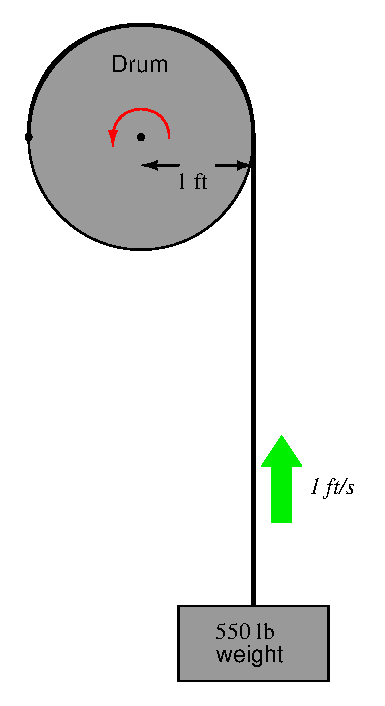
\includegraphics[width=15.5cm]{i01430x01.eps}$$

I dette tilfellet har vi en trommel med radius 1 fot som heiser en vekt på 550 pund med lineær hastighet 1 fot per sekund, altså definisjonen av én horsepower. Oversett lineær kraft og lineær hastighet til roterende kraft (dreiemoment) og roterende hastighet (RPM), og beregn deretter nødvendig $k$-faktor for å lage din egen ligning for dreiemoment/hastighet/horsepower.

\underbar{file i01430}
%(END_QUESTION)





%(BEGIN_ANSWER)

Dreiemomentet ($\tau$) i dette tilfellet er selvsagt 550 lb-ft, siden vekten på 550 pund virker på en momentarm som er 1 fot lang (trommelens radius). Alt vi trenger å gjøre er å oversette den vertikale hastigheten 1 fot/s til trommelrotasjon i enheten RPM, så har vi dataene vi trenger for å beregne $k$:

\vskip 10pt

$$\hbox{Trommelens omkrets } = \pi D = 2 \pi r = 6.283 \hbox{ ft}$$

Dette er kabelmengden som beveger seg i én omdreining av trommelen (1 rev = 6.283 ft), og denne likheten utgjør en konverteringsfaktor som vi kan bruke for å konvertere lineærhastigheten 1 ft/s til en rotasjonshastighet:

\vskip 10pt

$$\left({{1 \hbox{ ft}} \over \hbox{sec}} \right)  \left({{1 \hbox{ rev}} \over {6.283 \hbox{ ft}}}\right) \left( {{60 \hbox{ sec}} \over {1 \hbox{ min}}} \right) = 9.5493 \hbox{ RPM}$$

Dermed blir

$$P = k \tau S$$

$$1 \hbox{ hp}  = (k) (550 \hbox{ ft-lb}) (9.5493 \hbox{ RPM})$$

$$k = 0.0001904$$

$$P = 0.0001904 \tau S$$

$$\hbox{. . . eller . . .}$$

$$P = {{\tau S} \over 5252}$$

\noindent
Der,

$P$ = Aksel-effekt i horsepower

$\tau$ = Aksel-dreiemoment i lb-ft

$S$ = Akselhastighet i omdreininger per minutt (RPM)

\vskip 10pt

Litt tilfeldig er faktoren 5252 ganske nær antall fot i en mile (5280 fot = 1 mile). Det kan være nyttig som en tilnærming!

%(END_ANSWER)





%(BEGIN_NOTES)


%INDEX% Physics, torque: calculation problem
%INDEX% Physics, torque: shaft horsepower

%(END_NOTES)

